\documentclass[a4paper,10pt]{article}
\usepackage{titling}
\usepackage{fullpage}
\usepackage{times}
\usepackage{graphicx}
\usepackage{multicol}
\usepackage{float} %to place tables properly
\usepackage[table]{xcolor} %to color tables
\usepackage{placeins} %to place tables properly
\usepackage{hyperref} %for clickable links
\usepackage{listings} % <-- Add this line to include the listings package

\title{\vspace{40mm}\Large {Machine Learning Course} \vspace{0.2cm}
     \rule{\textwidth}{0.3pt} \vspace{0.1cm} % insert an horizontal line. Thickness 0.3pt
     \textbf{Fashion Image Classification} \vspace{0.0cm} %bold title
     \rule{\textwidth}{0.3pt}}

%information about author
\author{ Yasamin Hosseinzadeh Sani \vspace{0.1cm}\\
        \small Department of Computer Engineering\vspace{0.2cm}\\
        \small University of Pavia, Italy \vspace{0.2cm}\\
        }

\date{\today}

\begin{document}

\maketitle
\vspace{110mm}

\begin{abstract}
This report presents the implementation and evaluation of a convolutional neural network (CNN) for classifying fashion items into ten categories using grayscale images. The dataset comprises 70,000 images divided into training and test sets. The CNN model achieved a test accuracy of 82.4\%. This report details the data analysis, model training, evaluation, and visualization techniques used.
\end{abstract}

\tableofcontents

\section{Introduction}
Automating the classification of clothing items is a critical task for a warehouse specializing in recycling old clothes. This project aims to develop a machine learning model capable of accurately classifying images of clothing into ten predefined categories. By leveraging a convolutional neural network (CNN), the project aims to achieve high accuracy and provide insights into the model's performance through various evaluation metrics and visualizations.

\section{Goal}
The objective is to train and evaluate a convolutional neural network (CNN) to classify grayscale images of fashion items. The focus is on achieving high accuracy, understanding the model's behavior, and identifying areas for improvement.

\section{Data}

\subsection{Data Description}
The dataset consists of 70,000 grayscale images, each of 28x28 pixels, categorized into ten classes: T-shirt, Trouser, Pullover, Dress, Coat, Sandal, Shirt, Sneaker, Bag, and Ankle boot. The dataset is divided into a training set of 60,000 images and a test set of 10,000 images.

\subsection{Data Pre-processing}
Data pre-processing involved normalizing the pixel values to a range of 0 to 1 and reshaping the data to fit the input requirements of the CNN. Additionally, the labels were one-hot encoded for compatibility with the categorical cross-entropy loss function.

\begin{verbatim}
# Normalize the data
Xtrain = Xtrain.reshape(-1, 28, 28, 1) / 255.0
Xtest = Xtest.reshape(-1, 28, 28, 1) / 255.0

# One-hot encode the labels
Ytrain = to_categorical(Ytrain, num_classes=10)
Ytest = to_categorical(Ytest, num_classes=10)
\end{verbatim}

\subsection{Data Analysis}
Basic statistics and visualizations were generated to understand the dataset distribution and characteristics. The training data shape is (60000, 28, 28, 1), and the test data shape is (10000, 28, 28, 1). Each class has a substantial number of samples, ensuring a balanced dataset.

\begin{figure}[h]
\centering
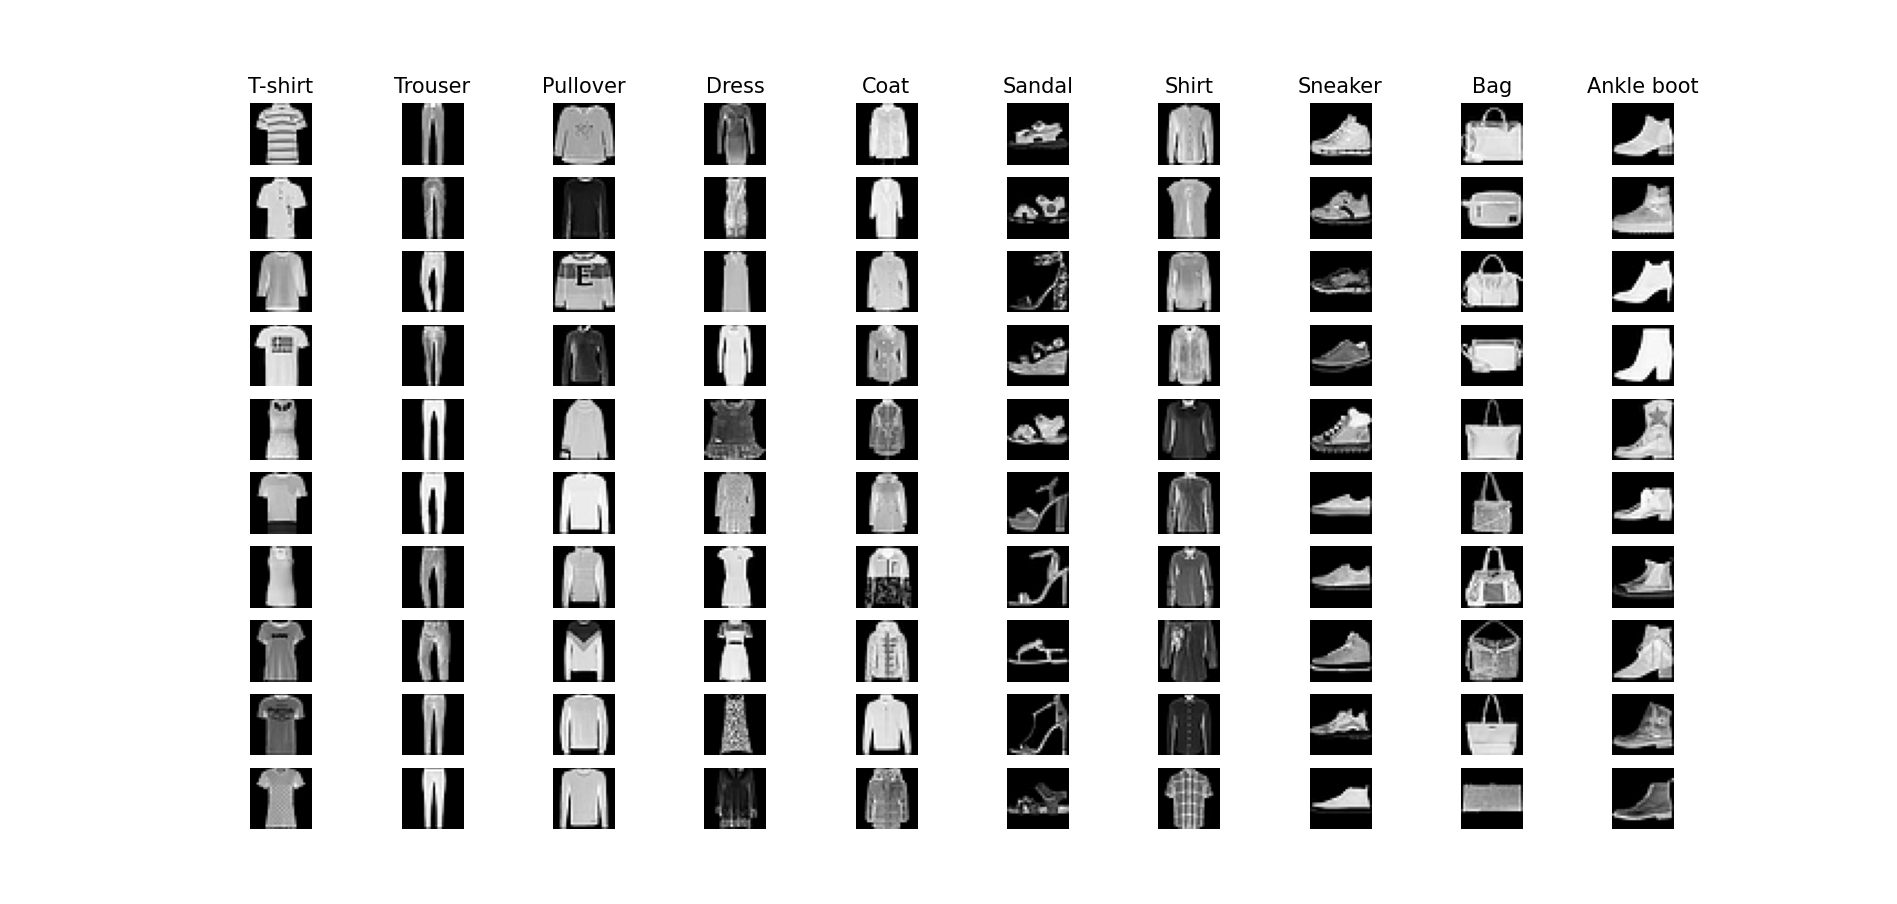
\includegraphics[width=0.8\textwidth]{1.png}
\caption{Examples of Different Classes}
\end{figure}

\section{Model Implementation}

\subsection{Convolutional Neural Network (CNN)}
The CNN architecture comprises two convolutional layers followed by max-pooling layers, a flatten layer, and two dense layers. The final layer uses softmax activation to output probabilities for the ten classes.

\begin{verbatim}
model = Sequential([
    Conv2D(32, kernel_size=(3, 3), activation='relu', input_shape=(28, 28, 1)),
    MaxPooling2D(pool_size=(2, 2)),
    Conv2D(64, kernel_size=(3, 3), activation='relu'),
    MaxPooling2D(pool_size=(2, 2)),
    Flatten(),
    Dense(128, activation='relu'),
    Dense(10, activation='softmax')
])

model.compile(optimizer='adam', loss='categorical_crossentropy', metrics=['accuracy'])
\end{verbatim}

\section{Training and Evaluation}

\subsection{Training the Model}
The model was trained for 10 epochs with a batch size of 128. The training process included logging the accuracy and loss for both training and validation datasets.

\begin{verbatim}
history = model.fit(Xtrain, Ytrain, epochs=10, validation_data=(Xtest, Ytest), batch_size=128)
\end{verbatim}

\subsection{Results}

\subsubsection{Training and Validation Accuracy and Loss}
The training and validation accuracy and loss curves provide insights into the model's learning process. The plots help identify overfitting, underfitting, and generalization performance.

\begin{figure}[h]
\centering
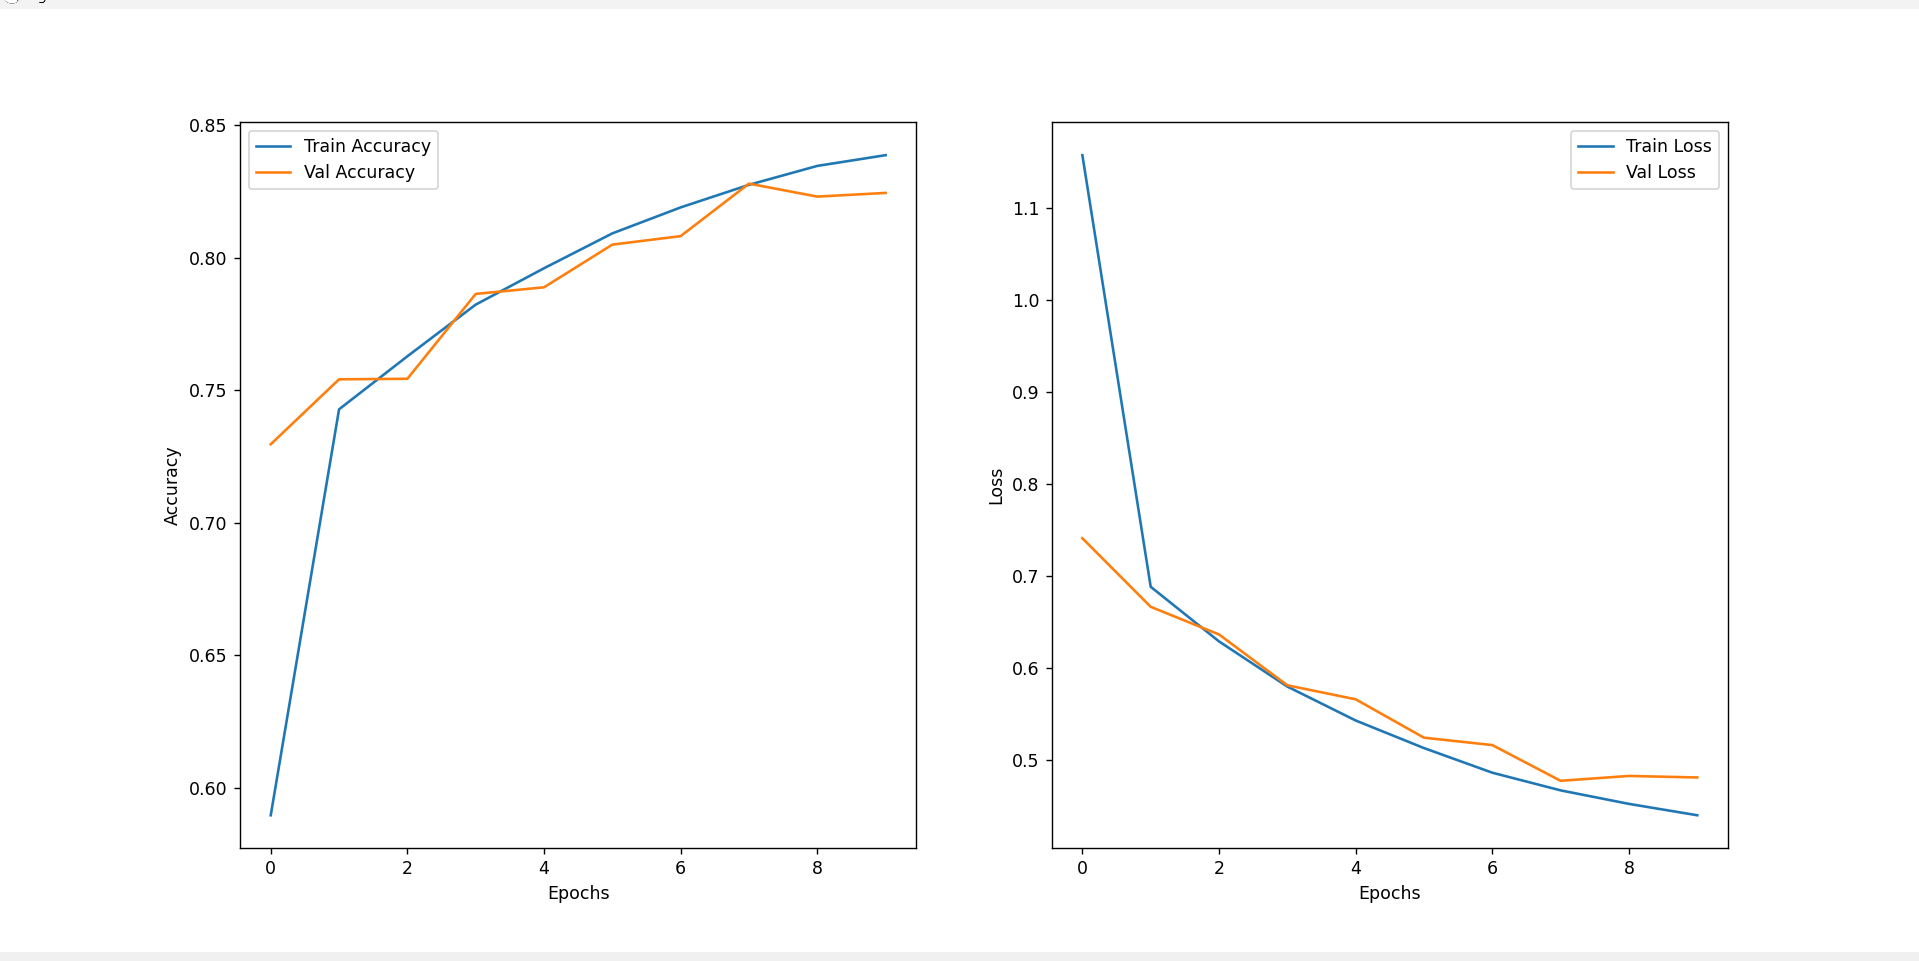
\includegraphics[width=0.8\textwidth]{2.png}
\caption{Training and Validation Accuracy and Loss}
\end{figure}

The accuracy and loss curves indicate that both training and validation accuracies improve steadily over the epochs. The final training accuracy reaches around 83.6\%, while the validation accuracy is slightly lower at 82.4\%. This close gap suggests that the model generalizes well to the test data.

The loss curves show a corresponding decrease in both training and validation losses, indicating that the model is learning effectively without significant overfitting.

\subsubsection{Confusion Matrix}
The confusion matrix provides a detailed breakdown of the model's performance across different classes, showing how often each class is correctly or incorrectly predicted.

\begin{figure}[h]
\centering
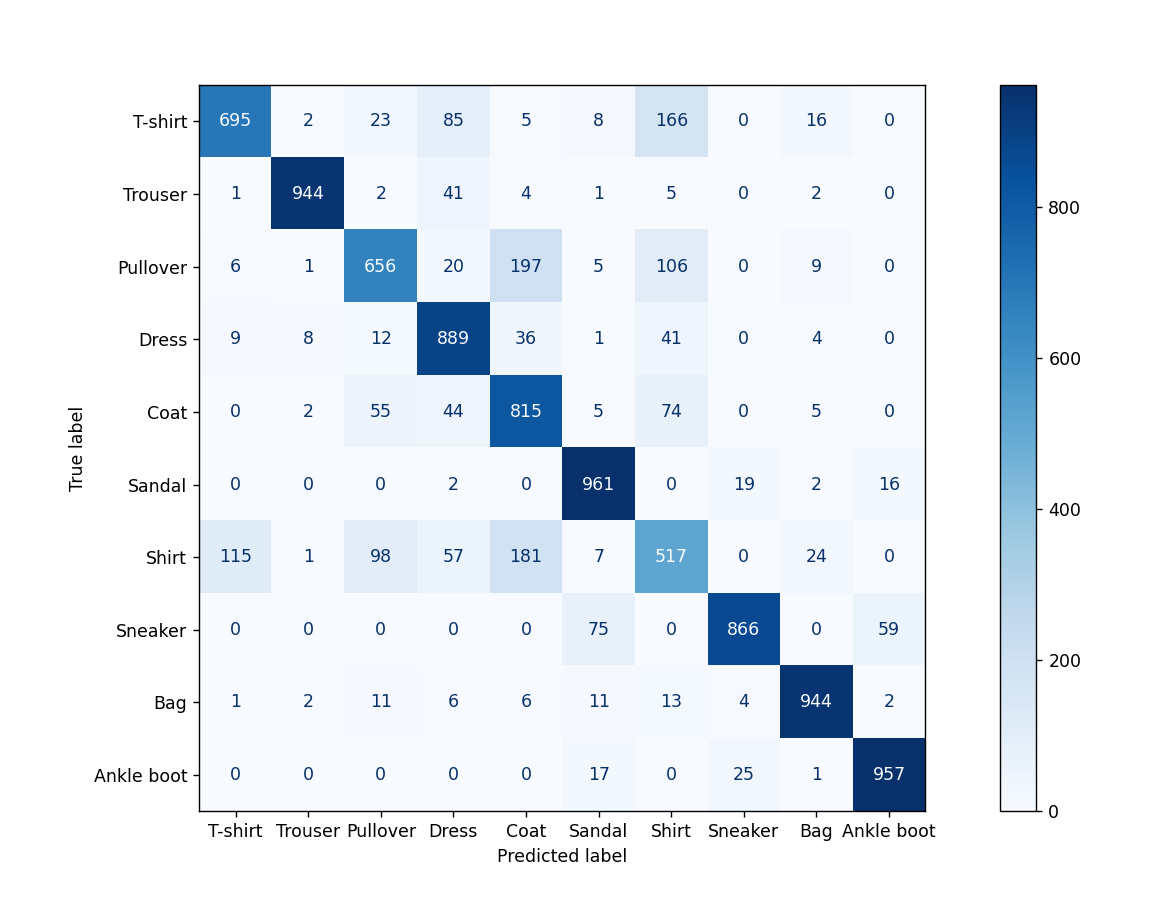
\includegraphics[width=0.8\textwidth]{3.png}
\caption{Confusion Matrix}
\end{figure}

The confusion matrix reveals the following insights:
\begin{itemize}
    \item The model performs exceptionally well on classes like "Trouser" and "Sandal," with high precision and recall. This indicates that the model is able to distinguish these items effectively.
    \item There is some confusion between similar classes, such as "Pullover" and "Coat," indicating that these items share visual similarities which the model finds difficult to distinguish.
    \item "Shirt" and "T-shirt" also have some misclassifications, which might be due to their overlapping features. This suggests a need for more feature differentiation or additional data to help the model learn the subtle differences.
\end{itemize}

\section{Best Models Analysis}

\subsection{Training Insights}
During training, various insights were gathered:
\begin{itemize}
    \item \textbf{Learning Rate:} A learning rate of 0.001 was found to be optimal for this model, providing a balance between convergence speed and stability. Too high a learning rate led to divergence, while too low a learning rate resulted in slow convergence.
    \item \textbf{Batch Size:} A batch size of 128 was chosen to ensure efficient use of computational resources while maintaining model performance. Larger batch sizes led to more stable updates but required more memory, while smaller batch sizes caused more variance in the updates.
\end{itemize}

\subsection{Most Misclassified Items}
Analyzing the most misclassified items helps identify common patterns and areas for improvement.

\subsubsection{Analysis of Misclassified Items}
The misclassified items provide several insights:
\begin{itemize}
    \item \textbf{Visual Similarities:} Items with visual similarities (e.g., "Pullover" and "Coat") are often misclassified, suggesting that the model may benefit from additional features or higher-resolution images. This could involve using deeper networks or ensemble methods to capture more complex patterns.
    \item \textbf{Ambiguous Features:} Some items have ambiguous features that make them hard to classify, even for humans. Addressing this might involve better feature engineering or leveraging more sophisticated models like transformers.
    \item \textbf{Data Quality:} Variations in image quality and angles can contribute to misclassifications, highlighting the need for more consistent data. Data augmentation techniques such as rotation, scaling, and flipping could be employed to make the model more robust to these variations.
\end{itemize}

\subsubsection{Overall Performance}
The model achieved a test accuracy of 82.4\%, which is satisfactory given the complexity of the task and the simplicity of the model architecture. The confusion matrix and misclassification analysis indicate that while the model performs well overall, there are specific areas (e.g., visually similar classes) that could benefit from further refinement. Future work could focus on improving these areas to enhance the model's performance.

\section{Conclusion and Future Work}
The CNN model performed well in classifying fashion items, achieving an accuracy of 82.4\%. The results indicate that the model is effective in recognizing most classes but faces challenges with visually similar items. Future work could involve:
\begin{itemize}
    \item \textbf{Experimenting with More Complex Architectures:} Adding more layers or using architectures like ResNet or VGG could improve performance. These architectures have proven effective in handling complex image classification tasks.
    \item \textbf{Data Augmentation:} Techniques like rotation, scaling, and flipping could help the model generalize better by exposing it to a wider variety of data.
    \item \textbf{Hyperparameter Tuning:} Further tuning of hyperparameters such as learning rate, batch size, and number of epochs could yield better results. Grid search or random search methods could be employed to find the optimal settings.
    \item \textbf{Transfer Learning:} Leveraging pre-trained models on similar datasets could enhance the model's accuracy and robustness. Fine-tuning a model pre-trained on a large dataset like ImageNet could provide a strong starting point for this task.
\end{itemize}


\section{References}
\begin{itemize}
    \item TensorFlow Documentation
    \item Scikit-learn Documentation
    \item "Deep Learning with Python" by François Chollet
\end{itemize}

\section{Instructions for Reproduction}
\begin{enumerate}
    \item Install the necessary libraries: \texttt{tensorflow}, \texttt{numpy}, \texttt{matplotlib}, \texttt{sklearn}.
    \item Load the data from \texttt{train.npz} and \texttt{test.npz}.
    \item Run the provided Python script \texttt{Mycode.py}.
\end{enumerate}

\textbf{I affirm that this report is the result of my own work and that I did not share any part of it with anyone else except the teacher.}


\end{document}
